\documentclass[conference]{IEEEtran}
\IEEEoverridecommandlockouts
\usepackage{blindtext, graphicx, caption, subcaption, cite}
\usepackage{amsmath,amssymb,amsfonts}
\usepackage[numbers]{natbib}
\usepackage{algorithmic}
\usepackage{textcomp}
\graphicspath{ {images/} }
\def\BibTeX{{\rm B\kern-.05em{\sc i\kern-.025em b}\kern-.08em
    T\kern-.1667em\lower.7ex\hbox{E}\kern-.125emX}}
    
\begin{document}
\title{Text Summerization Techniques}
\author{\IEEEauthorblockN{Anjana Tiha}
\IEEEauthorblockA{Department of Computer Science\\
University of Memphis, Memphis, TN\\
Email: atiha@memphis.edu}}
\maketitle
\begin{abstract}
This paper is focused with text summarization and currently popular text summarization techniques. This paper surveys on recent research on text summarization. 
\end{abstract}
\begin{IEEEkeywords}
Text Summerization, Machine Learning, Trending Text Summarization Techniques, Deep Learning.
\end{IEEEkeywords}
\section{Introduction}
Automatic text summarization is the process of generating concise and condensed, representation from one or more text documents data that fluently captures the core meaning and concept of the original text. There has been exponential growth of the world-wide web and social media usage causing dramatical increase in speed and the scaling of information dissemination. With such vast amount of accessible text documents on the Internet, it has become imperative to use text summarization in order to save time and effort in finding the right information. Summarization can be used for text, document, image and video. In image summarization the summarization system finds the most representative and important images. For videos, system tries to extract the important events from the long-time frame and uneventful context. Text summarization is a sub field of machine learning and data mining. There are mainly two approaches for generating automatic text or document summarization. Most common one is using extractive style, which extracts sentences essential to preserve the core idea of the text and combines them together to generate comprehensive text summery. This technique often use machine learning to score word, sentence or paragraph. Abstractive approach focuses more on the semantic meaning of the text and generates summery using natural language processing techniques.  

\section{Preprocessing}
For extractive summarization, preprocessing phase creates a representation of the original document. Usually, it identifies text boundaries and splits the text into paragraphs, sentences, and tokens. Sometimes, preprocessing requires special character, lower case and stop word removal along with stemming. 
\section{Extraction-based summarization}
After creating the intermediate representation of the original text using sentence boundary identification, special character, lower case and stop words removal and stemming, summarization system scores objects like words, sentences, paragraphs based on selected features. Sentences with highest scores are selected for summary.\\
Text summarization can be reduced to 3 steps:
\begin{enumerate}
\item Create an intermediate representation of the original text.
\item Sentence scoring.
\item Selecting high scoring sentences for generating summary.
\end{enumerate}
\subsection{Word Based Scoring}
There are different techniques for generating summery using word based scoring. In word based scoring, each sentence in a document is scored based on some selected features. After scoring based on features, cumulative score for each sentence is calculated for ranking. Highest scored sentences are selected to be in summary. Some of the common features for word based scoring includes word frequency, TF-IDF, upper case letter, proper noun and numerical data inclusive sentence.\\
\subsubsection{Word Frequency}
Assumes that words that occur frequently through the document are most important (Lloret \& Palomar, 2009; Gupta , 2011) and contain key information necessary for developing summarization. Each word of the document is scored based on weight derived from calculating frequency of it in the full text. Then cumulative score for each sentence is generated for all sentences present in the document. Finally, the sentences with higher scores are selected for document summary.\\
$$
TF/IDF = DN \times log(\frac{(1+tf)}{log(df)})
$$
\subsubsection{TF/IDF}
Text is first preprocessed by removing, hyperlinks, special characters, digits and stop words. Then words are stemmed to reduce to root words. Finally, TF-IDF is calculated for each sentence. Here, each sentence is treated as a document for term frequency calculation. Document frequency is calculated for each document. Sentences with highest cumulative scores are selected for summarization.\\
\subsubsection{Lexical Similarity}
Scores sentences based on idea that important sentences have strong chains words or lexical similarity (Gupta 2011; Barrera \& Verma).\\
\subsubsection{Upper Case}
Sentences with more importance are assumed to have more uppercase (Prasad et al., 2012 ) letters containing key information with proper which can be name, initials, highlighted words, proper nouns. The sentences with two or more upper case letters are assigned higher score and summarization is generated based on the highest ranked sentences.
$$CPTW =  \frac{NCW(j)}{NPW(j)}$$
where:\\
CPTW = Ratio of total first letter capital words present in the
sentence to the total number of words present in the sentence.\\
NCW = Number of first letter capital words.\\
NTW = Total number of words present in sentence.\\
$$UCf = \frac{CPTW(j)}{MAX(CPT(j))}$$
where, UCf = Uppercase feature value.\\
\subsubsection{Proper Noun}
Hypotheses on the concept that sentences with higher number of proper nouns are more important and hence, assigned higher scores (Fattah \& Ren, 2009).\\
\subsection{Sentence-based Scoring}
This approach is based on the features of the sentence itself.\\
\subsubsection{Cue-phrases}
Several cue phrases can identify most informative sentences in a document. For example, the sentences started with "In summary", "In conclusion" contain the concise summery. Also, emphasis is given by phrases such as, "Most importantly", "Most significantly", "Particularly". Phrases like "according to the study", "in our finding" contains factual data. Also, domain-specific phrases or terms can be good indicators of significant content of a text (Gupta et al., 2011).
$$
CP = \frac{CPS}{CPD}
$$
where,\\
CP = Cue-phrase score.\\
CPS = Number of cue-phrases in a sentence.\\
CPD = Total number of cue-phrases in a single document.\\
\subsubsection{Sentence Position}
The position of a sentence can be crucial indicator of its relative importance. For example, the most important sentences tend to come at the beginning or end of a document or near the title text. There are couple of approaches for position based sentence scoring. One is giving weight 1 to the first N sentences (Satoshi et al., 2001) and the rest of the sentences are given 0 weight. In paper (Barrera \& Verma, 2012), sentences have been scored based on three positions, sentences closer to the title, sentences at the beginning of the paragraph and sentences at the end of paragraph. Sentences closer to these 3 positions were given more weight and hence more likely to be selected for summary. Also, for domain specific document summarization, domain knowledge can be used for automated summary.\\
\subsubsection{Sentence Resemblance To The Title}
Sentence resemblance to the title is the vocabulary overlap between this sentence and the document title (Satoshi et al., 2001). Words in the title is considered most important and contains key terms that convey the central concept of the document. Sentence with high resemblance with the title is have an overlapping vocabulary with title. The concept centrality embodied in title vocabulary and thus can help retain important sentences.
$$
Score = Ntw/T
$$
where,\\
Ntw = Number of title words in sentence.\\
T = Number of words in the title.\\
\subsubsection{Sentence Length}
This scoring method penalizes sentences that are or too long or too short, as  they are not considered as an ideal selection. Length is counted by number of words in a sentence.
$$
Score = Length(s) \times (Average Sentence Length)
$$
\subsubsection{Sentence Inclusion of Numerical Data}
Sentences containing numerical data is considered more important and containing crucial information for informative summary. Hence, sentences with numerical data is likely to be included (Abuobieda et al., 2012;) in the text summary.\\

\subsection{Graph-based Scoring:}
In graph-based methods the score is generated by the analyzing relationship among sentences in a document. When a sentence refers to another it generates a link with an associated weight between them. The weights are used to generate the scores of a sentence.\\\\
Text is preprocessed by removing digits, special characters, stop words and converting them to lower case. After initial preprocessing, stemming is done to reduce to root words. In the graph based approach, all the sentences are considered as a node in a graph. Based on shared or similar information like overlapping vocabulary, two nodes are connected. The nodes or sentences with higher cardinality is considered more important for summarization.\\\\\\\\
Some graph based techniques are:\\
\subsubsection{Text Rank}
It extracts the important keywords from a text document and determines the weight of the “important” of words within the entire document by using a graph-based model. Sentences with higher rank are selected.
\subsubsection{Cluster Based Method}
Text documents can have an organizational pattern and key information can be extracted by identifying locations/sections of important segment of the document. In this approach, each document is divided into multiple segments or clusters and objects (word, sentence) in each segment are given weights based on term importance (TF-IDF or other features). Next, each segment is ranked by calculating the overall importance score for all the objects present in each segment. Segments with highest scores are then selected for final summary.
\subsubsection{Chalanges Of Extractive Summarization}
Problem with extractive summarization is that it can lead to lack of coherency. Also, summery especially unit sentences can be too long to understand the concept accurately. Often document can contain counter information. Presenting them in summery can lead to ambiguity and confusion beating the original motivation behind summarization.  Also, key information could get ignored due to selection of scoring method. 
\section{Dataset}
From Ferreira \cite{Ferreira} experiment:
\subsubsection{CNN Dataset} The CNN corpus developed by Lins and colleagues (Lins et al., 2012)  400 texts assigned to 11 categories: Africa, Asia, business, Europe, Latin America, Middle East, US, sports, tech, travel, and world news.
\subsubsection{Blog summarization dataset} Hu and colleagues (Hu, Sun, \& Lim, 2007, 2008) collected data from two blogs, Cosmic Variance (http://cosmicvariance.com) and Internet Explorer Blog (http://blogs.msdn.com/i.e./). From those blogs, 100 posts, 50 from each blog, were randomly chosen to form the evaluation dataset.
\subsubsection{SUMMAC dataset} The SUMMAC Corpus was elaborated with University of Edinburgh, as part of the SUMMAC conference organizer group.183 papers on Computation and Language, obtained from the repository LANL (Los Alamos National Laboratory) maintained by Cornell University Library.
\section{Results}
From Ferreira experiment:\\
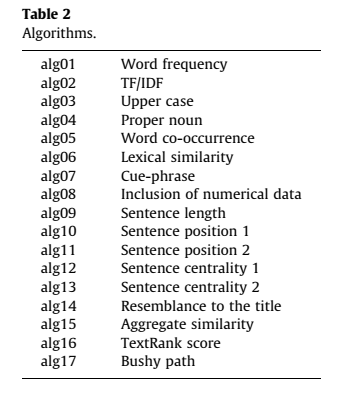
\includegraphics[scale=.6]{algs}
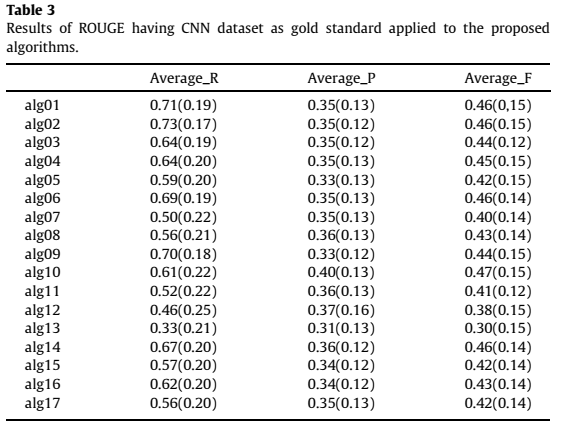
\includegraphics[scale=.5]{cnn1}
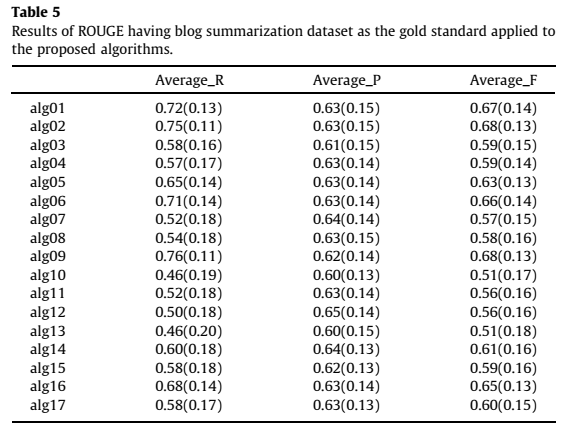
\includegraphics[scale=.5]{blg1}
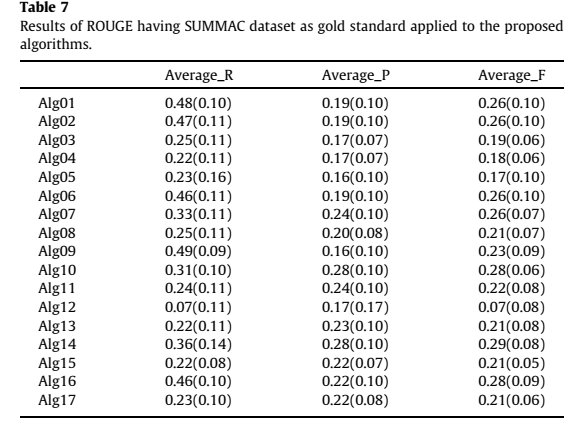
\includegraphics[scale=.5]{summac1}
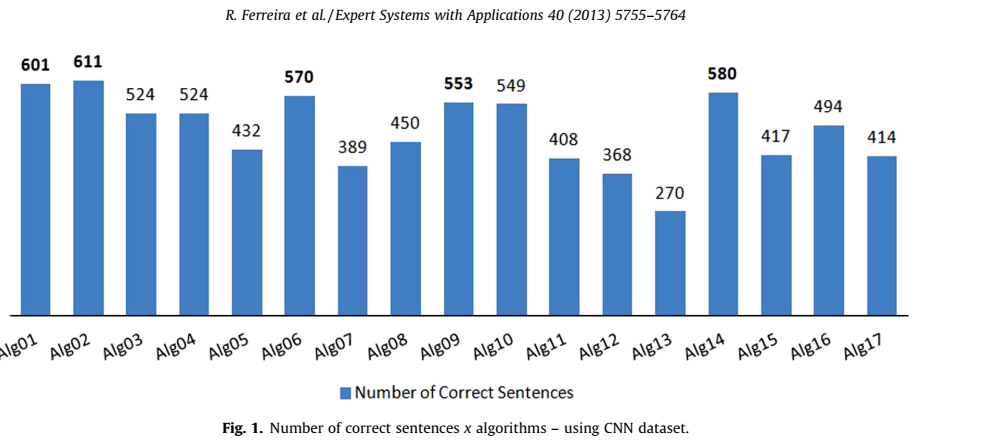
\includegraphics[scale=.35]{cnn2}
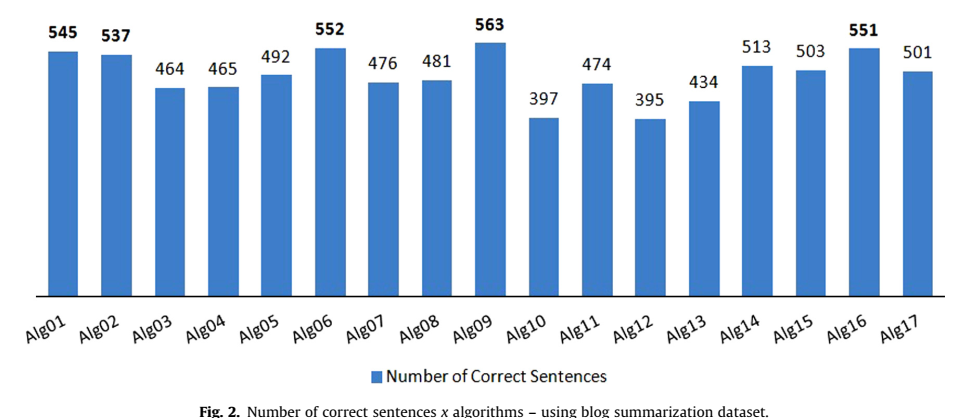
\includegraphics[scale=.35]{blg2}
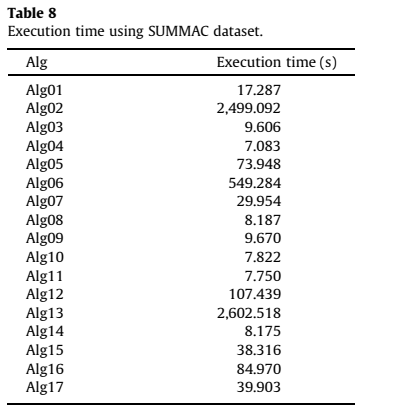
\includegraphics[scale=.4]{summac2}
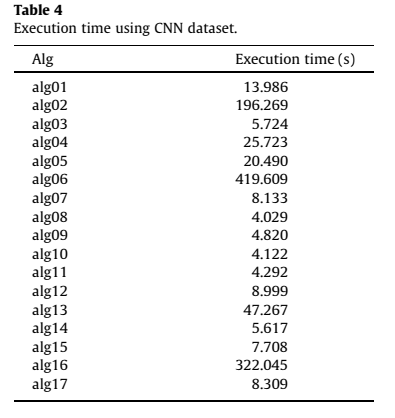
\includegraphics[scale=.4]{cnn3}
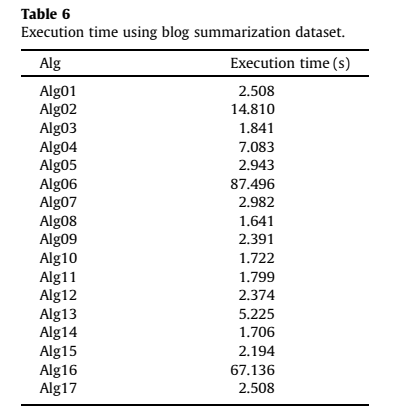
\includegraphics[scale=.4]{blg3}
\section{Comarative Performance From Paper}
Among all the algorithm, word frequency, TF-IDF, sentence length seemed to perform better(Assessing sentence scoring techniques, Rafael).
\section{Abstraction-based summarization}
In abstraction based approach, summarization system paraphrases segments of the source document. Abstraction based techniques can generate more condensed text than extraction techniques. Abstractive summaries try to improve the coherence among sentences by eliminating redundancies and clarifying the contest of sentences. But, this requires usage of natural language generation technology, which is still in growth stage. While there has been some recent work in abstractive summarization, the majority of summarization systems are using extractive methods.
\section{Conclusion}
For automatic text summarization, extraction based techniques are mostly used. Some recent work has been done on abstractive text summarization. Semantic based approach has also been experimented. But as it requires better NLP techniques, it is still work in progress. Recurrent neural network has also been applied for summarization recently.  
\begin{thebibliography}{1}
\bibitem{Vishal}
Gupta, Vishal, and Gurpreet Singh Lehal. "A survey of text summarization extractive techniques." Journal of emerging technologies in web intelligence 2.3 (2010): 258-268.
\bibitem{Ferreira}
Ferreira, Rafael, et al. "Assessing sentence scoring techniques for extractive text summarization." Expert systems with applications 40.14 (2013): 5755-5764.
\bibitem{Alexander}
Rush, Alexander M., Sumit Chopra, and Jason Weston. "A neural attention model for abstractive sentence summarization." arXiv preprint arXiv:1509.00685 (2015).
\bibitem{Gupta}
Gupta P, Pendluri VS, Vats I. Summarizing text by ranking text units according to shallow linguistic features. InAdvanced Communication Technology (ICACT), 2011 13th International Conference on 2011 Feb 13 (pp. 1620-1625). IEEE.
\bibitem{Lloret}
Balahur A, Lloret E, Boldrini E, Montoyo A, Palomar M, Martínez-Barco P. Summarizing threads in blogs using opinion polarity. InProceedings of the workshop on events in emerging text types 2009 Sep 17 (pp. 23-31). Association for Computational Linguistics.
\bibitem{Verma}
Barrera A, Verma R. Combining syntax and semantics for automatic extractive single-document summarization. Computational Linguistics and Intelligent Text Processing. 2012:366-77.
\bibitem{Fattah}
Fattah MA, Ren F. GA, MR, FFNN, PNN and GMM based models for automatic text summarization. Computer Speech \& Language. 2009 Jan 31;23(1):126-44.
\bibitem{Kulkarni}
Shardan R, Kulkarni U. Implementation and evaluation of evolutionary connectionist approaches to automated text summarization.
\bibitem{Lloret}
Lloret E, Palomar M. Text summarisation in progress: a literature review. Artificial Intelligence Review. 2012 Jan 1;37(1):1-41.
\end{thebibliography}
\end{document}





